\documentclass[12pt]{article}

%packages
\usepackage[utf8]{inputenc}
\usepackage{sectsty}
\usepackage{enumitem}
\usepackage{hyperref}
\usepackage{natbib}
\usepackage{graphicx}

%settings
\sectionfont{\normalsize}
\setlength{\bibhang}{0.5in}
\bibliographystyle{apalike}

%document
\title{Letter of Inquiry}
\author{Journal of Quantitative Description: Digital Media}

\begin{document}

\maketitle

\section*{Research question}
How reliable is the NewsGuard database of domain trustworthiness ratings over time and language contexts?

\section*{Why is it important for digital media research?}
On social media, misinformation is widely visible \citep{lazerScienceFakeNews2018} and embedded in growing partisan sorting and intergroup conflict~\citep{gonzalez-bailonAsymmetricIdeologicalSegregation2023a}. To study these dynamics on digital platforms, it is imperative for computational social scientists to have access to reliable and valid tools that enable them to identify misinformation. A prominent way to track misinformation is to use a list of domains. The organization NewsGuard offers the most comprehensive database of domain trustworthiness ratings. Despite its increasing popularity~\citep[for example,][]{robertsonUsersChooseEngage2023a,lasserSocialMediaSharing2022a}, the database was created as a tool for brand security rather than research, which is why access is not public and rather expensive. 

This proposal outlines a descriptive analysis of the content of the NewsGuard database over time and across countries, focusing on three questions:
\begin{itemize}
    \item \textbf{How volatile are trustworthiness ratings, e.g. how often do ratings change or domains vanish?} This is important to estimate whether using an older database will distort results.
    \item \textbf{How reliable and complete is the provided information, particularly for non-US countries?} A recent study has shown high agreement of NewsGuard with other expert-rated lists in the U.S. context~\citep{linHighLevelCorrespondence2023}, but an assessment for other countries is missing. 
    \item \textbf{How can other information be used for misinformation research?} For each domain, NewsGuard rates journalistic quality criteria, topics, political slants, and labels AI-generated content. This information might shed light on aspects of misinformation beyond binary true/false labels.
\end{itemize}
By describing the database, we outline potential pitfalls and recommendations for digital media research. We also want to empower misinformation researchers to make informed decisions about whether the substantial expense associated with acquiring access to NewsGuard is necessary for their research. 

\section*{What is being described?}
NewsGuard experts regularly assess the trustworthiness of news outlets. As of September 20, 2023, the database contains 10,993 trustworthiness assessments. Each assessment includes:
\begin{itemize}
    \item The domain and overall trustworthiness (between 0 and 100).
    \item Binary labels (yes/no) for nine journalistic quality criteria constituting the trustworthiness rating. Criteria are ``Regularly corrects or clarifies errors'' (12.5 points) or ``Gathers and presents information responsibly'' (18 points)\footnote{See \href{https://www.newsguardtech.com/ratings/rating-process-criteria/}{https://www.newsguardtech.com/ratings/rating-process-criteria/} for a full list.}
    \item The language and country associated with the domain,  covering nine countries as well as a ```global'' label, and five languages (English, Italian, French, German, Spanish). Most assessments are from the US (66\%), followed by global domains (12\%), Great Britain (5\%), Italy (5\%), Canada (4\%), France (4\%) and Germany (3\%).
    \item Topics covered (e.g., ``local news'', ``political news'', ``health information'') and political orientation (left/right).
    \item A flag indicating whether the outlet frequently posts AI-generated content.
\end{itemize}

\section*{How is the sample constructed?}
NewsGuard rates outlets based on web traffic data, claiming that they have reviewed domains accounting for 95\% of online engagement. The organization sometimes adds outlets they deem influential or that changed domains. NewsGuard saves hourly snapshots of the database, allowing us to track changes going back to March 2019, when the organization started to operate. 
Notably, NewsGuard is not a blacklist. In fact, close to 60\% of the domains have an overall rating of over 60 and are therefore considered ``trustworthy''(see Fig.~\ref{fig:fig1}) for the distribution. 
\begin{figure}
    \centering
    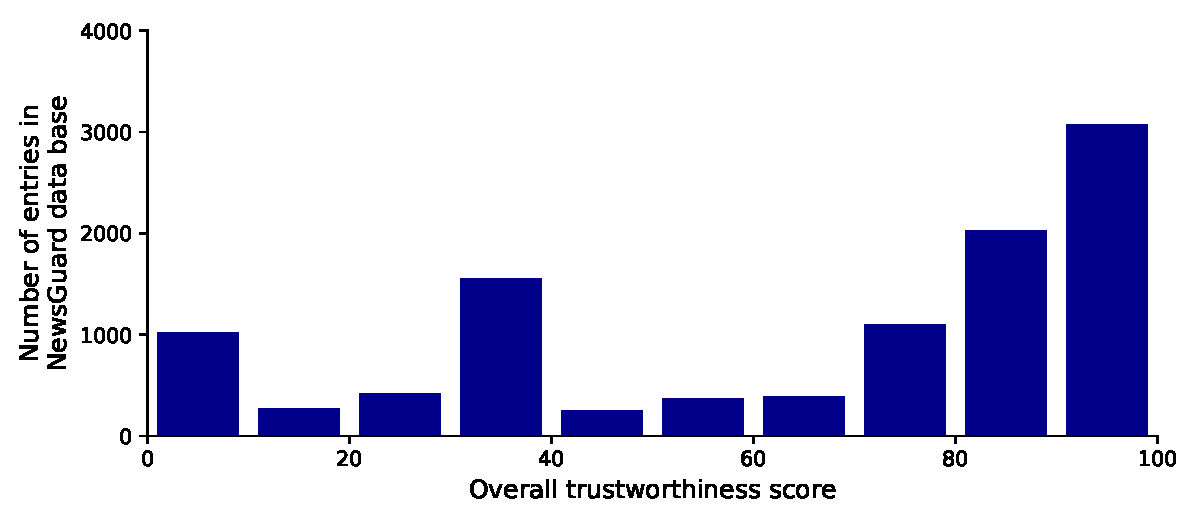
\includegraphics[width=\textwidth]{NewsGuard_histogram.pdf}
    \caption{Distribution of domain trustworthiness contained in the NewsGuard database as of September 20, 2023.}
    \label{fig:fig1}
\end{figure}

\bibliography{newsguard-review.bib}
\end{document}